\chapter{Domain Driven Design}
\section{Ubiquitous Language}

\begin{table}[t]
	\centering
	\noindent\makebox[\textwidth]{
		\begin{tabular}{ c | c }
			Domänenexperte (KeePass/1Password) & Implementierung (Morik) \\
			\hline
			Password & PlaintextPassword \\
			Password & EncryptedPassword \\
			Entry/Item & Entry \\
			UUID & EntryId \\ 
			Title & EntryName \\
			User Name & Login \\
			Vault & EntryRepository \\
			Password Generator & PasswordGenerator \\
			Length of generated password & PasswordLength \\
			? & PasswordEncrypter \\
			? & PasswordDecryper \\
		\end{tabular}
	}
	\caption{Ubiquitous Language Gegenüberstellung}
	\label{tab:ubiquitous_language}
\end{table}

Die Analyse der Ubiquitous Language ergab die zuvor genannten Programmteile, deren Bezeichnungen mit denen anderer Passwortmanager verglichen werden. KeePass unterscheidet in der Ubiquitous Language nicht zwischen den zwei von uns identifizierten Arten von Passwörtern, nämlich PlaintextPassword und EncryptedPassword. Stattdessen werden diese zwei Umstände meist mit Adverben beschrieben ("sensitive data is stored encryptedly", "make sensitive data available unencryptedly") oder mithilfe mehrerer Substantive ("passwords as plain-text"). Da wir im Source Code weder mit Adverben noch mit unnötig langen Konstrukten aus mehreren Substantiven arbeiten wollen, wir jedoch trotzdem eine Unterscheidung der beiden Zustände eines Passworts benötigen, haben wir uns für die beiden genannten Varianten entschieden. Was das Entry angeht, so verwenden wir den gleichen Begriff wie KeePass (1Password zieht hier Item vor). Was die EntryId angeht, so verwenden wir keine UUID, da wir nur Entries verwalten und demnach keine eindeutige Kennung über mehrere Tabellen hinweg benötigen. Das Präfix "Entry" vor der Id dient dem besseren Nachvollziehen von was es die Id ist. Das Gleiche gilt für das Präfix des EntryName. Hier haben wir uns für Name statt wie KeePass für Title entschieden, da wir dies für eindeutiger halten. Außerdem haben wir uns gegen User Name entschieden und haben stattdessen Login gewählt als Begriff, da unser Passwort Manager darauf abzielt dem Benutzer beim Anmelden zu helfen. Aus diesem Grund kann im Feld Login die konkrete Zeichenkette gespeichert werden, die der Benutzer zum Anmelden braucht, sei es tatsächlich der Benutzername oder aber die Email Adresse. Entsprechend uneingeschränkt sollte auch die Bezeichnung dieses Feldes sein, was bei User Name nicht der Fall ist. 1Password nennt den Ort, an dem die Passwörter gespeichert werden den Vault. Wir haben uns stattdessen für EntryRepository entschieden, um zum einen klar zu machen, dass es sich um einen Aufbewahrungsort handelt und zum anderen eindeutig festzulegen, dass dies der Aufbewahrungsort speziell für Entries ist. Dies beseitigt sämtliche Fragen, was genau dort aufbewahrt wird. Beim PasswordGenerator jedoch sind wir uns einig mit der Bezeichnung von KeePass. Was die PasswordLength jedoch angeht, war uns die Formulierung von KeePass zu lang, weshalb wir uns die Präposition \enquote{of} und das Adjektiv \enquote{generated} gespart haben. Außerdem ist das Adjektiv sowieso überflüssig, da nur beim Generieren der Passwörter überhaupt explizit eine Länge gesetzt werden muss, denn wenn der Benutzer das Passwort selbst eingibt, so legt er diese implizit fest. Weder KeePass noch 1Password benennen die Teile ihrer Software, die die Daten ver- und entschlüsseln. Stattdessen ist die Rede von "encrypted data" und "decrypted data". Da Passwörter die einzigen Felder sind, die von uns ver- und entschlüsselt werden, haben wir uns dafür entschieden die dafür zuständigen Programmteile mit PasswordEncryptor und PasswordDecryptor zu bezeichnen, sodass wir trotzdem die von KeePass und 1Password verwendeten Wortstämme verwenden, daraus jedoch Substantive machen.

Um die Ubiquitous Language des Programms auch außerhalb des Source Codes zu verwenden, haben wir ebenfalls die Spalten der Datenbank an die festgelegten Begriffe angepasst. Dies kann in \autoref{fig:DDDDatabase} beobachtet werden.

\begin{figure}[ht]
	\centering
	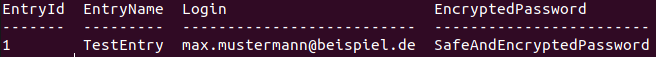
\includegraphics[width=1.0\textwidth]{Bilder/DDD_column_names.png}
	\caption{Datenbank-Spaltennamen nach Ubiquitous Language}
	\label{fig:DDDDatabase}
\end{figure}

\section{Value Objects}
Das erste Value Object ist das \href{https://github.com/moorts/Morik/blob/main/src/application/PlaintextPassword.h}{\textit{PlaintextPassword}}, welches das vom Benutzer eingegebene abzulegende Passwort beinhaltet bevor es verschlüsselt wird beziehungsweise nachdem es entschlüsselt wird. Es handelt sich dabei um ein Value Object, da es sich um das gleiche PlaintextPassword handelt wenn der Benutzer zwei mal die gleiche Zeichenkette eingibt. Das \href{https://github.com/moorts/Morik/blob/main/src/application/EncryptedPassword.h}{\textit{EncryptedPassword}}, das das Passwort beinhaltet nachdem es verschlüsselt ist, gilt ebenfalls als Value Object. Dies gilt aus dem gleichen Grund wie beim PlaintextPassword, also dass die gleiche Zeichenkette auch die Gleichheit des Objekts impliziert. Auch die \href{https://github.com/moorts/Morik/blob/main/src/application/PasswordLength.h}{\textit{PasswordLength}}, die die Länge des zu generierenden Passworts speichert, ist ein Value Object, da eine gleiche PasswordLength bedeutet, dass die Passwörter gleich lang sind. Außerdem gilt der \href{https://github.com/moorts/Morik/blob/main/src/application/EntryName.h}{\textit{EntryName}} als Value Object, der den Namen, welchen der Benutzer für den Eintrag vergibt, speichert. Hierbei handelt es sich ebenfalls um ein Value Object, da die gleiche eingegebene Zeichenkette bedeutet, dass es sich um den gleichen Namen für den Eintrag handelt. Auch der vom Benutzer optional hinzugefügte \href{https://github.com/moorts/Morik/blob/main/src/application/Login.h}{\textit{Login}} eines Entrys gilt als Value Object, ebenfalls aus dem Grund dass die gleiche Zeichenkette bedeutet, dass das Objekt das Gleiche ist. Zu guter Letzt gilt auch die \href{https://github.com/moorts/Morik/blob/main/src/application/EntryId.h}{\textit{EntryId}} als Value Object, die die ID des Entrys speichert. Hier gilt, dass der gleiche Integer Wert schlussfolgern lässt, dass es das gleiche Objekt der Klasse EntryId ist.

\section{Entities}
Ein \href{https://github.com/moorts/Morik/blob/main/src/application/Entry.h}{\textit{Entry}} beschreibt einen konreten Eintrag in der Datenbank. Der Entry beinhaltet die ID des Eintrags, den Namen des Eintrags, einen optionalen Login und das verschlüsselte Passwort. Man stelle sich Folgendes vor. Der Benutzer löscht einen Entry und erstellt danach einen neuen. Bei dem neuen Entry vergibt er den gleichen Namen, Login und das gleiche Passwort wie bei dem zuvor gelöschten Entry. Handelt es sich deshalb um den selben Entry wie der vorherige? Nein, denn der wurde gelöscht. Darum ist der Entry eine Entity und kein Value Object.

\section{Aggregate}
Es gibt genau ein Aggregat. Dieses Aggregat beinhaltet einen Entry, eine EntryId, einen EntryName, einen Login und ein EncryptedPassword. Diese Teile sind als Aggregat zu betrachten, da sie immer gemeinsam von Interesse sind. Ein Benutzer möchte nicht einfach irgend ein Passwort wissen ohne den zugehörigen Namen des Eintrags zu kennen. Die Aggregat-Root ist dabei der Entry, wobei über die EntryId des Entrys auf das jeweilige Aggregat zugegriffen wird.

\section{Repositories}
Da es nur ein Aggregat gibt, gibt es ebenfalls genau ein Repository. Dieses Repository ist die \href{https://github.com/moorts/Morik/blob/main/src/application/EntryRepository.h}{\textit{EntryRepository}} und stellt den Zugriff auf die Datenbank dar, die die Einträge des Benutzers persistiert. Das EntryRepository liefert demnach vorhandene Entries zurück, speichert neue Entries, löscht nicht mehr benötigte und passt Werte eines Entrys an neue Werte an.

\section{Domain Services}
Der Generator für neue Passwörter (\href{https://github.com/moorts/Morik/blob/main/src/application/PasswordGenerator.h}{\textit{PasswordGenerator}}), sowie die Verschlüsselung eines PlaintextPasswords (\href{https://github.com/moorts/Morik/blob/main/src/application/PasswordEncryption.h#L11}{\textit{PasswordEncryptor}}) und die Entschlüsselung eines EncryptedPasswords (\href{https://github.com/moorts/Morik/blob/main/src/application/PasswordEncryption.h#L22}{\textit{PasswordDecryptor}}) werden als Domain Services realisiert.
